\section{Blockchain Data Fetching}\label{section:data-model}

Explain briefly the hardware used in the test?

A crucial aspect of any blockchain based application with end user interaction lies within the responsiveness. The guest client application provides an interface that is never blocked for user interaction, except when the user chooses to switch to another cryptocurrency wallet. The data abstraction and storage layer discussed in [ref] underwent multiple iterations during the development process. The following section discusses some performance benchmarks, along with their respective impact on the usability of the application. It also mentions some specific code changes that lead to improvements in certain benchmarks. All benchmarks have been evaluated on an Intel i5-7600 CPU with a clock speed of 3.5GHz and 4 individual cores. The application was accessed through the Chromium browser.

\subsection{Baseline - Event Loading}\label{section:bl-events}
In order to get a solid baseline for event loading times, the application was tasked with fetching event data for three different events, with two, five, and ten ticket types (TT) each. For this experiment no caching mechanism has been used (\textit{cold start}). The loading times are shown in \ref{img:baseline1}. A higher number of ticket types leads to consistently longer loading times, when all other variables such as the number of Solidity events are isolated.

\begin{figure}[H]
    \centering
    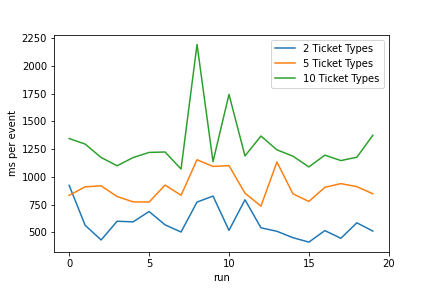
\includegraphics[width=14cm]{images/plot1.png}
    \caption{Baseline event loading times \protect\footnotemark}
    \label{img:baseline1}
\end{figure}

Figure \ref{tab:baseline1} shows mean and average loading times over the course of 20 consecutive runs. The median is consistently lower across this and all later on discussed experiments. This may be attributed to ...
From Table \ref{tab:baseline1} one can extrapolate a difference of approximately \textit{320ms} in loading times when going from two to five ticket types. The absolute increase in time is slightly lower when going from five to ten ticket types.  

\begin{table}[ht]
\centering
\begin{tabular}{|c|c|c|c|c|c|}
\hline
 & \textbf{Mean [ms]} & \textbf{Median [ms]} \\ \hline
2 TT & 587.03               & 551.39         \\ \hline
5 TT & 904.23               & 878.72         \\ \hline
10 TT & 1281.94               & 1191.82         \\ \hline
\end{tabular}
\caption{Baseline event loading time statistics}
\label{tab:baseline1}
\end{table}

\subsection{Baseline - User Interactions}\label{section:bl-user}


The second baseline was measured in order to capture the effect of user actions. For this one event with one, two, and four ticket types respectively was deployed. There were 50 user accounts funded with test Ethers, each of witch bought a ticket and made an aftermarket listing. Figure \ref{img:baseline2} shows the loading times for this scenario. The loading times were higher compared to Figure \ref{img:baseline1}. This is expected behaviour due to the moderate amount of user induced Solidity events.
\begin{figure}[H]
    \centering
    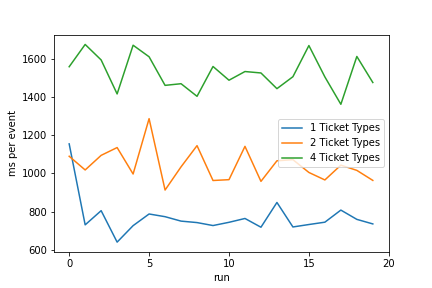
\includegraphics[width=14cm]{images/plot2.png}
    \caption{Baseline User Interactions \protect\footnotemark}
    \label{img:baseline2}
\end{figure}

Table \ref{tab:baseline1} displays the mean and the average loading times over the course of 20 runs.


\begin{table}[ht]
\centering
\begin{tabular}{|c|c|c|c|c|c|}
\hline
 & \textbf{Mean [ms]} & \textbf{Median [ms]} \\ \hline
1 TT & 770.80             & 744.55      \\ \hline
2 TT & 1043.78             & 1026.26       \\ \hline
4 TT & 1526.70               & 1515.72        \\ \hline
\end{tabular}
\caption{Baseline user interaction loading times statistics}
\label{tab:baseline1}
\end{table}


\subsection{Account Switching}\label{section:account-switching}

One feature specifically enabled by the data abstraction layer is immediate user account switching. Figure \ref{img:user_int} shows an experiment on a blockchain state with 20 events deployed. One user account was configured to buy a ticket for each of these events and make an aftermarket listing as well. On a cold start it took around three seconds to load all of the users data, which although covered with a loading screen, is a notable loading time. The warm start, using the locally cached data from the abstraction layer, was able to consistently load all of the users tickets and display them within around 0.2 seconds.

\begin{figure}[H]
    \centering
    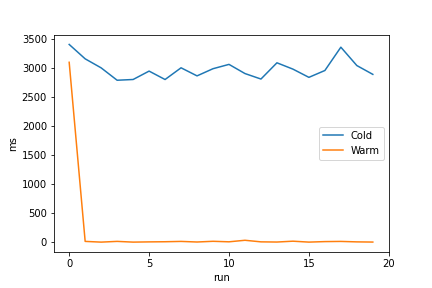
\includegraphics[width=14cm]{images/plot3.png}
    \caption{Ethereum user account switching times \protect\footnotemark}
    \label{img:user_int}
\end{figure}

\begin{table}[ht]
\centering
\begin{tabular}{|c|c|c|c|c|c|}
\hline
 & \textbf{Mean [ms]} & \textbf{Median [ms]} \\ \hline
Cold & 2978.96            & 2963.11     \\ \hline
Warm & 164.99           &  8.98      \\ \hline
\end{tabular}
\caption{Ethereum user account switching times statistics}
\label{tab:baseline1}
\end{table}


\subsection{Preloading in Detail}\label{section:eval-preloading}


In this last evaluation, an event with a large number of user interactions over the course of 858 blocks was prepared on the blockchain. The application was tasked with completely fetching the event's data while having the information from all Solidity events up to increasing block number cached in the abstraction layer. Figure \ref{img:caching} shows the loading times for each level of cached data. The labels show the block number up until which the data was cached (lower means more data to load). Block 858 was the last block with new Solidity events. 

\begin{figure}[H]
    \centering
    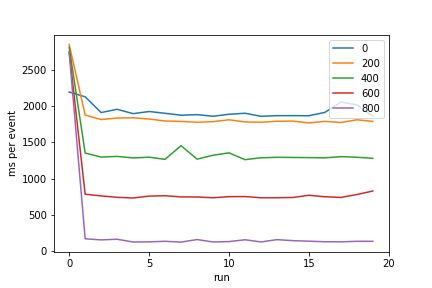
\includegraphics[width=14cm]{images/plot4.png}
    \caption{User Switching Times \protect\footnotemark}
    \label{img:caching}
\end{figure}

Table \ref{tab:caching} shows the mean and average loading times for each stage. The benefit of local caching and an efficient data abstraction manifests itself in this evaluation. With 50\% of the data stored locally, the loading time decreases almost linearly and with over 90\%, the application can load an event's data within a fraction of a second.
 
\begin{table}[ht]
\centering
\begin{tabular}{|c|c|c|c|c|c|}
\hline
\textbf{Starting Block} & \textbf{Mean[ms]} & \textbf{Median [ms]} \\ \hline
0   & 2978.96         & 1900.95    \\ \hline
200 & 1933.94         &  1794.26   \\ \hline
400 & 1855.97         &  1294.84    \\ \hline
600 & 1381.26         &  750.0    \\ \hline
800 & 268.80          &  133.41     \\ \hline
\end{tabular}
\caption{User Switching Times statistics}
\label{tab:caching}
\end{table}

\subsection{Discussion}\label{section:eval-discussion}

While the numerical results of the evaluation have displayed the benefits of the local caching mechanisms within the guest client, there are some additional concerns to mention. First and foremost, all of the experiments, if not explicitly stated otherwise, have been conducted on a local blockchain. This means that the average loading times are not representative of what should be expected on a truly distributed ledger. We argue that this is a further case for the client side caching mechanism as the introduced network overhead could be significantly reduced by only ever requesting from the blockchain what has never been loaded to the client before, or what has been manually removed from the client by the user.  